\documentclass[dvipsnames]{../../../../AritzhClass}

\usepackage{array}
\usepackage{arydshln}

\makeatletter
\renewcommand*\env@matrix[1][*\c@MaxMatrixCols c]{%
  \hskip -\arraycolsep
  \let\@ifnextchar\new@ifnextchar
  \array{#1}}
\makeatother

\usetikzlibrary{calc}
\lstset{
	language=C,
	showstringspaces=false,
	numbers=none,
	xleftmargin=0cm
}

\izenburua{Bonba}
\azpiizenburua{Proiektuaren Txostena}
\smalltitle{Bonba: Txostena}
\ikasgaia{Ingeniaritza Informatikoa: KE}
\author{Aritz Lopez}
\data{\today}

\begin{document}

\izenburuorrialdea

\tableofcontents

\pagebreak

\section{Proiektuaren enuntziatua}

Nintendo DS-rako \textit{100 doors} jokuaren motako ate bat diseinatu eta programatu, DS-aren pantaila, teklatua eta denboragailua erabiliz.

\section{Proiektuaren definizioa: Bonba}

Ebazpenerako pentsatu dugun atea zeran datza: Ukimen pantailan bonba bat agertuko da, 5 kablerekin, eta jokalariak kable egokia moztu behar izango du 10 segunduren barruan, bonba lehertu ez dadin. Jokoaren berjokagarritasuna honakoan datza: jokalariak kable desegokia pultsatuz gero, berriro saiatzeko aukera izango du (\textit{A} tekla pultsatuz gero); honela, aurreko kable bera pultsatu beharko du. Bestela, galtzean \textit{B} tekla pultsatzen badu, ausazko beste kable bat izango da moztu behar dena.

\section{Kontzeptu-mapa}

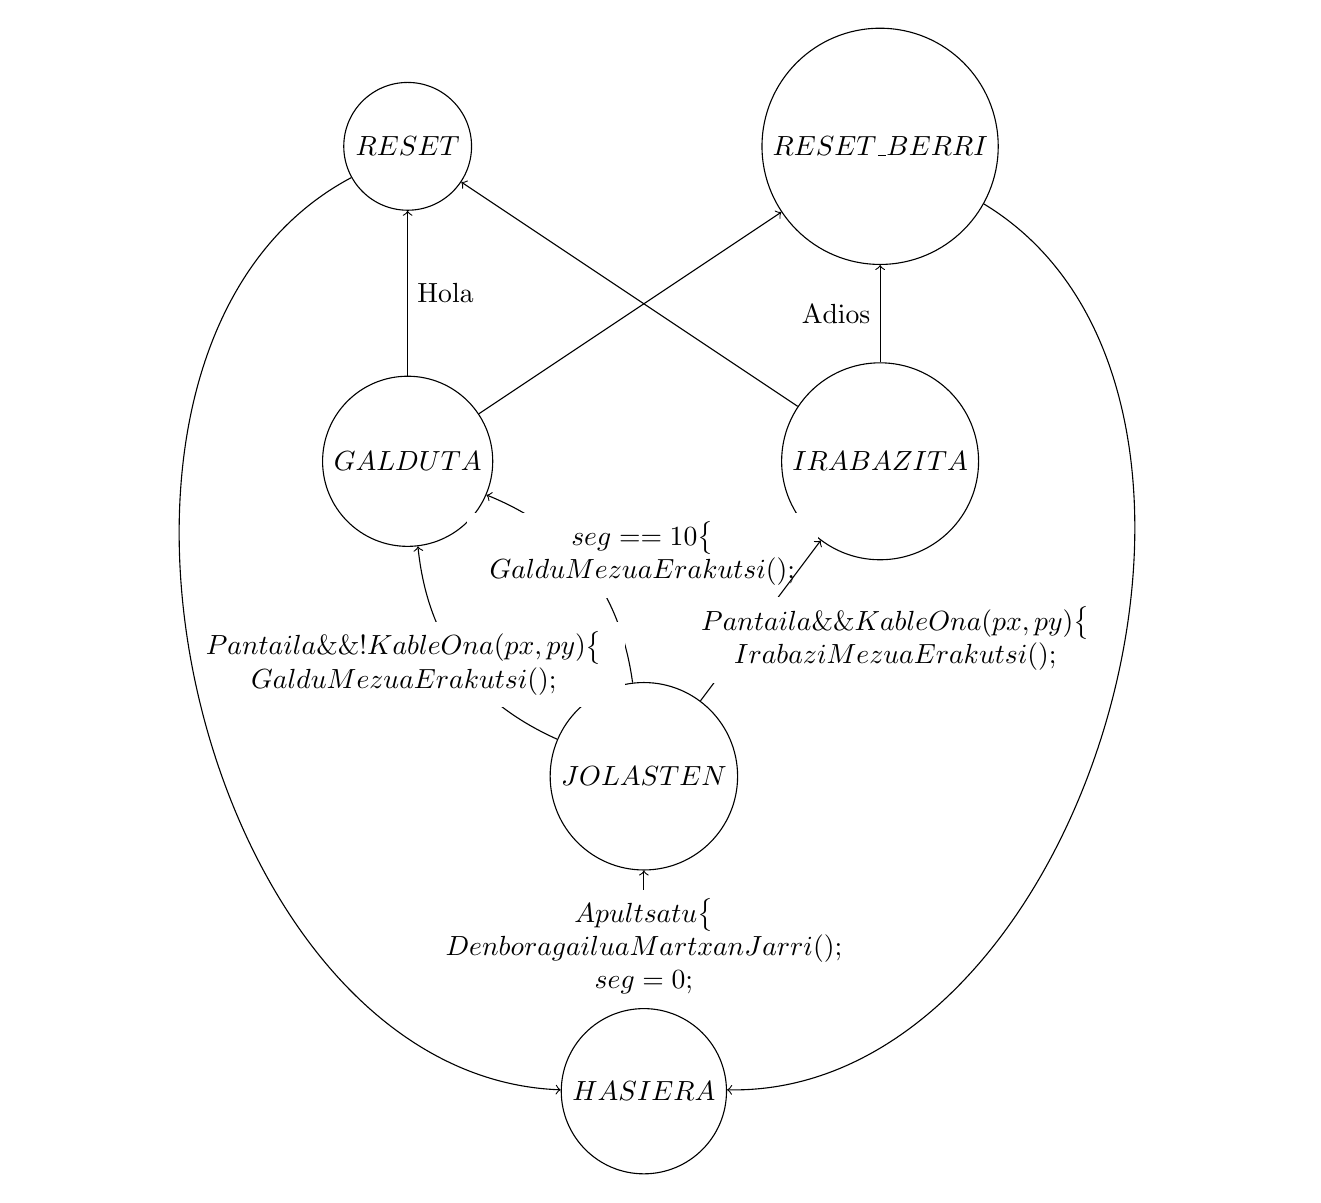
\begin{tikzpicture}
\node(0) at (3,0)[shape=circle,draw]	{$HASIERA$};
\node(1) at (3,4)[shape=circle,draw]    {$JOLASTEN$};
\node(2) at (0,8)[shape=circle,draw]    {$GALDUTA$};
\node(3) at (6,8)[shape=circle,draw]	{$IRABAZITA$};
\node(4) at (0,12)[shape=circle,draw]	{$RESET$};
\node(5) at (6,12)[shape=circle,draw]	{$RESET\_BERRI$};
\path [->]
  (0) edge node [above, preaction={fill, white}, yshift=-25] {$\begin{array}{c}
   A\text{ pultsatu}\big\{ \\
   \text{DenboragailuaMartxanJarri();} \\
   \text{seg=0;}
  \end{array}$} (1)
  (1) edge [bend right=30]  node [below, preaction={fill, white},yshift=20,xshift=20] {$\begin{array}{c}\text{seg==10} \big\{ \\ \text{GalduMezuaErakutsi();}\end{array}$} (2)
  (1) edge [bend left=30]  node [below, preaction={fill, white},yshift=15,xshift=-20] {$\begin{array}{c}\text{Pantaila \&\& !KableOna(px, py)} \big\{ \\ \text{GalduMezuaErakutsi();}\end{array}$} (2)
  (1) edge node [above, right, preaction={fill, white}, yshift=-7, xshift=-30] {$\begin{array}{c}\text{Pantaila \&\& KableOna(px, py)} \big\{ \\ \text{IrabaziMezuaErakutsi();}\end{array}$} (3)
  (2) edge node [above, right] {Hola} (4)
  (2) edge node [above] {} (5)
  (3) edge node [above] {} (4)
  (3) edge node [above, left] {Adios} (5)
  
  (4) edge [bend right=75]  node [below] {} (0)
  (5) edge [bend left=75]   node [below] {} (0)
  %(0) edge [loop above]    node [above] {} ()
  ;
\end{tikzpicture}

\end{document}
